% latexmk -pdflatex='lualatex' -pdf treelogo.tex
\documentclass{standalone}
\usepackage{fontspec}
% \setmainfont[
    % Extension      = .ttf,
    % Ligatures      = TeX,
    % BoldFont       = LiberationSans-Bold,
    % ItalicFont     = LiberationSans-Italic
  % ]{LiberationSans-Regular}

% \setmainfont[ Extension=.ttf ]{AlegreyaSansSC-Bold}
% \setmainfont[ Extension=.ttf ]{LiberationSans-Bold}
% \setmainfont[ Extension=.otf ]{NimbusSans-Bold}
% \setmainfont[ Extension=.ttf ]{AlegreyaSansSC-ExtraBold}
% \setmainfont[ Extension=.ttf ]{OdorMeanChey-Regular}
% \setmainfont[ Extension=.ttf ]{Inconsolata-Bold}
\setmainfont[ Extension=.ttf ]{DejaVuSans-Bold}

% \setmainfont[ Extension=.ttf ]{Hind-Bold}
% \setmainfont[ Extension=.ttf ]{Heebo-Bold}

\usepackage{tikz}
\usetikzlibrary{decorations.text}  
\usepackage{calc}
\usepackage{graphicx}

\newsavebox\mybox


\begin{document}   

\centering
\sbox\mybox{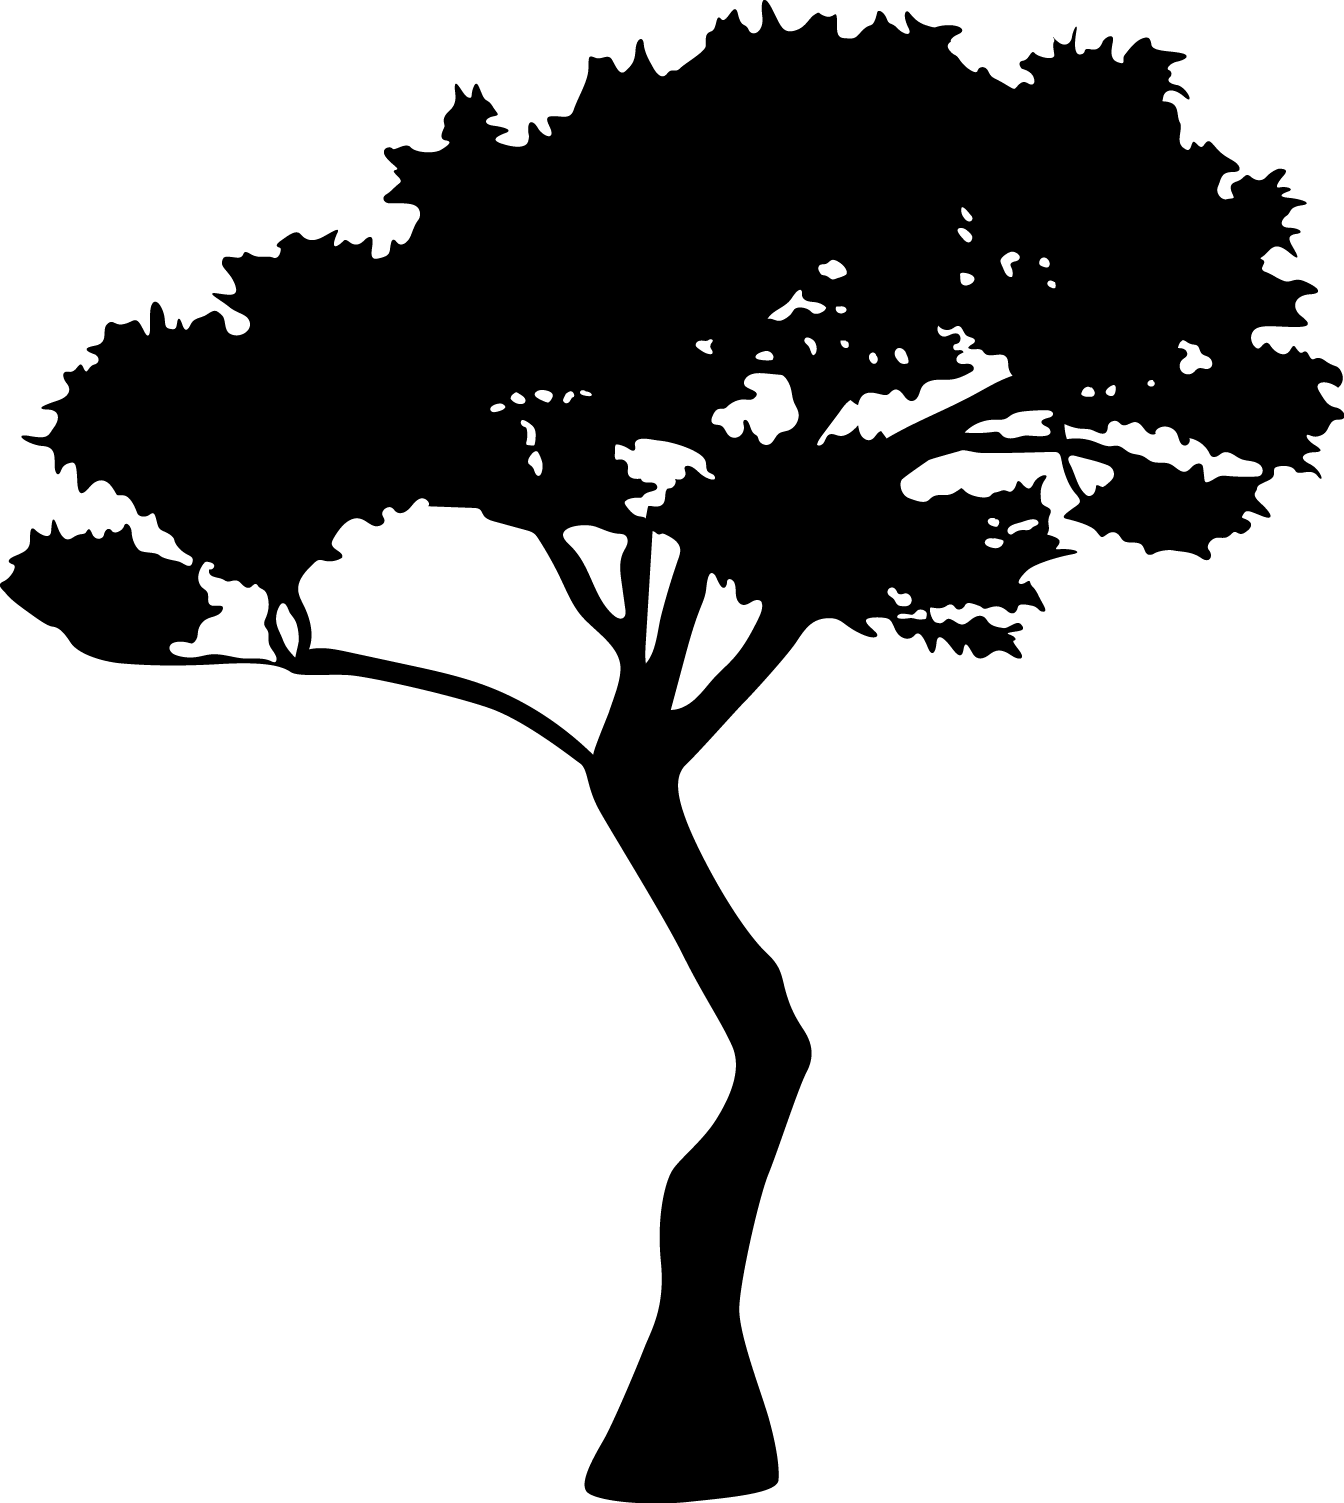
\includegraphics[scale=.5]{tree.png}}%
\begin{tikzpicture}[x=\wd\mybox/1344, y=\ht\mybox/1503]
    \node[anchor=south west,inner sep=0pt] at (0,0) {\usebox\mybox};
    % \draw (700,751) circle [radius=800]; % Circle around which text is based
  % \node[draw] at (0,0) {DejaVu};
    \path (700,751) circle [radius=800];
\begin{scope}[shift={(700,751)}]
% \fontsize{45pt}{45pt}\selectfont
\fontsize{40pt}{40pt}\selectfont
\path[font = \sffamily, decoration = {text along path, text = {CCR},
    text align = {align = center}, raise = -1ex}, decorate]
        (-170:550) arc (-170:-110:550);
% \fontsize{35pt}{35pt}\selectfont
\fontsize{30pt}{30pt}\selectfont
\path[font = \sffamily, decoration = {text along path, text = {La Jolla}, text align = {align = center}, raise = -.6ex}, decorate] (-80:650) arc (-80:20:650);
% \fontsize{25pt}{25pt}\selectfont\bf
% \path[font = \sffamily, decoration = {text along path, text = {LA JOLLA}, text align = {align = center}, raise = -.8ex}, decorate] (-80:650) arc (-80:20:650);
\end{scope}
\end{tikzpicture}

\end{document}
